%----------------------------------------------------------------------------
%----------------------------------------------------------------------------
%				    	SETUP
%----------------------------------------------------------------------------
%----------------------------------------------------------------------------

\documentclass[12pt]{article}

%----------------------------------------------------------------------------
%			  	   PACKAGES
%----------------------------------------------------------------------------

%% Fonts and Symbols
%% --------------------------
\usepackage[T1]{fontenc}			% better font encoding
\usepackage[utf8]{inputenc}		% better font encoding
%\usepackage[usenames,dvipsnames,svgnames,table]{xcolor}		% allow colour
\usepackage{amsmath,amssymb,amsthm,textcomp, xfrac}		% math symbols, etc
%\usepackage{color}
\usepackage[hidelinks]{hyperref}	% hyperlinks, see config in LAYOUT AND STYLING


%% Graphics
%% --------------------------
\usepackage{graphicx}			% allow insertion of images
\graphicspath{ {./graphics/} }		% the relative path to the graphics folder
\usepackage{subfigure}			% allows subfigures (a), (b), etc
%\usepackage{tikz}				% vector graphics
%\usepackage{pgfplots}			% plots in vector graphics


%% Tables
%% --------------------------
\usepackage{booktabs}			% better tables, discourages vertical rulings
%\usepackage{tabularx}
%\usepackage{enumerate}		
\usepackage{multicol}			%allow multi columns


%% Layout Alteration
%% --------------------------
\usepackage{lastpage}
\usepackage{fancyhdr}			% see config in LAYOUT AND STYLING
\usepackage{fullpage}			% set full page margins
%sideways figures
\usepackage{rotating}
%\usepackage{pdflscape}
%\usepackage{parskip}			% disable indents

%% Units
%% --------------------------
\usepackage{siunitx}			% has S (decimal align) column type
\sisetup{input-symbols = {()},  % do not treat "(" and ")" in any special way
         group-digits  = false} % no grouping of digits
%\sisetup{load-configurations = abbreviations}
%\sisetup{per-mode = symbol}
%\usepackage{cancel}

%% Misc
%% --------------------------
%\usepackage{mhchem}			% chemistry


%----------------------------------------------------------------------------
%		     MACROS AND COMMANDS
%----------------------------------------------------------------------------

%type Y - even column width - centered
% must include tabularx package
%\newcolumntype{Y}{>{\centering\arraybackslash}X}	

% Defines a new command for the horizontal lines, change thickness here
\newcommand{\HRule}{\rule{\linewidth}{0.5mm}} 	

% ???
\newcommand{\linia}{\rule{\linewidth}{0.5pt}}

% scientific notation  use \e
\providecommand{\e}[1]{\ensuremath{\times 10^{#1}}}

% diferential
\def \d {\ensuremath{\mathrm{d}}}

%----------------------------------------------------------------------------
%		   	LAYOUT AND STYLING
%----------------------------------------------------------------------------

% custom footers and headers
% must include fancyhdr package
\pagestyle{fancy}
\lhead{}
\chead{}
\rhead{}
\lfoot{}
\cfoot{\thepage\ of \pageref{LastPage}}
\rfoot{}
\renewcommand{\headrulewidth}{0pt}
\renewcommand{\footrulewidth}{0pt}


%%section style
%\usepackage{titlesec}
%\titleformat{\section}[runin]
%{\normalfont\bfseries}
%{\thesection.}{.5em}{}[]
%
%\titleformat{\subsection}[runin]
%{\normalfont\bfseries}
%{\thesubsection}{.5em}{}[]
%\setcounter{secnumdepth}{0} %dont number sections

%\hypersetup{
%%    	colorlinks=false, 		% set true if you want colored links
%   		linktoc=all,     			% set to all if you want both sections and subsections linked
%%  		linkcolor=blue,  			% choose some color if you want links to stand out
%}


%----------------------------------------------------------------------------
%----------------------------------------------------------------------------
%				   DOCUMENT
%----------------------------------------------------------------------------
%----------------------------------------------------------------------------

\begin{document}

%----------------------------------------------------------------------------
%				    TITLE PAGE
%----------------------------------------------------------------------------

\begin{titlepage}

\center
 
% Header
\textsc{\LARGE University of Victoria}\\[1cm] 	% Name of your university/college
\textsc{\Large ELEC 250}\\[0.5cm] 			% Major heading such as course name
\textsc{\large Linear Circuits I}\\[0.5cm] 		% Minor heading such as course title


% Lab Title
\HRule \\[0.4cm]
{ \huge \bfseries Lab 2 - Phasor Analysis}\\[0.2cm] % Title of your document
\HRule \\[1.5cm]
 
 
%Lab Instructor Details
\begin{minipage}{0.7\textwidth}
\begin{flushleft} 

\large\emph{Instructor:} \\
Dr. Nikitas \textsc{Dimopoulos} \\
\vspace{12 pt}
\emph{Teaching Assistant:} \\
Zhen \textsc{Liu}

\end{flushleft}
\end{minipage}
~
%% No content here, but it keeps the alignment of the instructor/TA
%% box correct.
%% Consider revising.
\begin{minipage}{0.1\textwidth}
\begin{flushright} \large
%Dr. Barbara \textsc{Sawicka} \\
\vspace{12 pt}
%\emph{Teaching Assistant:} \\
%Vahid \textsc{Moradi}
\end{flushright}
\end{minipage}\\[2cm]


% Lab members
\Large Clayton \textsc{Kihn}
\large V00794569	\\
\Large Yves \textsc{Senechal}
\large V00213837	\\
\Large Tyler \textsc{Stephen}
\large V00812021	\\
A01 - B01\\[1.5cm] 


% Date
{\large \today}\\ % Date, change the \today to a set date if you want to be precise

% Logo
\begin{figure}[b]	 % put logo at bottom of the page
	\centering
	\includegraphics[scale=0.3]{UVic_logo}
\end{figure}

\end{titlepage}

%----------------------------------------------------------------------------
%			  TABLE OF CONTENTS
%----------------------------------------------------------------------------

%\tableofcontents
%\pagebreak

%\listoffigures
%\pagebreak

%----------------------------------------------------------------------------
%				    BODY
%----------------------------------------------------------------------------

\section{Object}\label{sec:object}
This lab will study the steady-state responses of an RC and RL circuit when exposed to a purely sinusoidal voltage source. The current response and the phase shift of current relative to voltage will be calculated and compared with measured values.

\section{Results}\label{sec:results}
An Agilent 33220A signal generator was used to create the sinusoidal voltage source used in this lab. A peak-to-peak voltage of 10.5 V was used for both circuits. Different frequencies were used in each section and is discussed further in sections \ref{sec:rc} and \ref{sec:rl}.

An Agilent DSOX-2012A oscilloscope was used to analyze the maximal current and phase shift.

\subsection{RC Circuit}\label{sec:rc}
The circuit was connected as show in figure \ref{fig:rc} using selectable capacitor and resistor boxes provided in the lab. A 5 nF capacitor was used in the circuit. A sinusoidal voltage source with a frequency 10 kHz was applied to the circuit.

\begin{figure}[h]
	\centering
	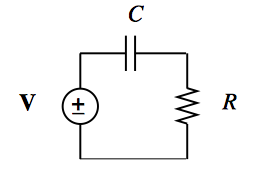
\includegraphics[scale=0.6]{RC_circuit}
	\caption{The RC circuit used in the lab}
	\label{fig:rc}
\end{figure}

The expected phase shift, with current leading voltage, is given by equation \eqref{eqn:rc_theta}, where $\omega = 2\pi f$. The expected maximum current is given by equation \eqref{eqn:rc_current}.

\begin{equation}
	\tan { \theta  } =\left( \frac { 1 }{ \omega RC }  \right) 
	\label{eqn:rc_theta}
\end{equation}

\begin{equation}
		I_{max} = \frac{V_{max}}{\sqrt{R^2 + (\frac{1}{C\omega})^2} }
		\label{eqn:rc_current}
\end{equation}

\pagebreak
The calculated and measured values of the current ($I$) and phase shift ($\theta$) are summarized in table \ref{table:rc}.

\begin{table}[h]
	\centering
	\begin{tabular}{c c c c c}
		\toprule
		&				\multicolumn{2}{c}{Calculated}	& \multicolumn{2}{c}{Measured}	\\
		\cline{2-5}
		$R$ (k$\Omega$)	& $I$ (mA) 	& $\theta$ ($^\circ$) 	& $I$ (mA) 	& $\theta$ ($^\circ$) \\
		\hline
		1				& 3.15		& 72.56					& 3.10			&	70.89	\\
		5				& 1.77		& 32.48					& 1.76			&	31.12	\\
		10				& 1.00		& 17.67					& 0.98			&	14.89	\\
		\toprule
	\end{tabular}
	\caption{Calculated and measured values in the RC circuit}
	\label{table:rc}
\end{table}

\subsection{RL Circuit}\label{sec:rl}
The circuit was connected as shown in figure \ref{fig:rl}. The resistor box was reused and discrete inductors were obtained from the lab (see tables \ref{table:rl_calc} and \ref{table:rl_meas}). The frequency of the voltage source was set to 500 kHz.

\begin{figure}[h]
	\centering
	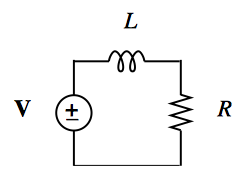
\includegraphics[scale=0.6]{RL_circuit}
	\caption{The RL circuit used in the lab}
	\label{fig:rl}
\end{figure}

The expected phase shift of current with respect to voltage is given by equation \eqref{eqn:rl_theta}. The negative sign indicates that voltage will lead current. The expected maximum current is given by equation \eqref{eqn:rl_current}.

\begin{equation}
	\tan { \theta  } =\left( \frac { -\omega L }{ R }  \right) 
	\label{eqn:rl_theta}
\end{equation}

\begin{equation}
		I_{max} = \frac{V_{max}}{\sqrt{R^2 + L^2\omega^2}}
		\label{eqn:rl_current}
\end{equation}

\pagebreak
Calculated values for each pairing of resistor and inductor is summarized in table \ref{table:rl_calc}. Measured results are presented in table \ref{table:rl_meas}.

\begin{table}[h]
	\centering
	\begin{tabular}{c S S S S S S S S}
		\toprule
		& \multicolumn{2}{c}{$1 \mu$H}	& \multicolumn{2}{c}{$220 \mu$H} & \multicolumn{2}{c}{$470 \mu$H} & \multicolumn{2}{c}{$1000 \mu$H} \\
		\cline{2-9}
		$R$ (k$\Omega$)	& \multicolumn{1}{c}{$I$ (mA)} 	& \multicolumn{1}{c}{$\theta$ ($^\circ$)} 	& \multicolumn{1}{c}{$I$ (mA)} 	& \multicolumn{1}{c}{$\theta$ ($^\circ$)}	& \multicolumn{1}{c}{$I$ (mA)} 	& \multicolumn{1}{c}{$\theta$ ($^\circ$)}	& \multicolumn{1}{c}{$I$ (mA)} 	& \multicolumn{1}{c}{$\theta$ ($^\circ$)} \\
		\hline
		1		& 10.50	& -0.18	& 8.64	& -34.65& 5.89	& -55.89& 3.18	& -72.34\\
		5		& 2.10	& -0.04	& 2.08	& -7.87	& 2.01	& -16.45& 1.78	& -32.14\\
		10		& 1.05	& -0.02	& 1.05	& -3.95	& 1.04	& -8.40	& 1.00	& -17.44\\
		\toprule
	\end{tabular}
	\caption{Calculated values in the RL circuit}
	\label{table:rl_calc}
\end{table}

\begin{table}[h]
	\centering
	\begin{tabular}{c S S S S S S S S}
		\toprule
		& \multicolumn{2}{c}{$1 \mu$H}	& \multicolumn{2}{c}{$220 \mu$H} & \multicolumn{2}{c}{$470 \mu$H} & \multicolumn{2}{c}{$1000 \mu$H} \\
		\cline{2-9}
		$R$ (k$\Omega$)	& \multicolumn{1}{c}{$I$ (mA)} 	& \multicolumn{1}{c}{$\theta$ ($^\circ$)} 	& \multicolumn{1}{c}{$I$ (mA)} 	& \multicolumn{1}{c}{$\theta$ ($^\circ$)}	& \multicolumn{1}{c}{$I$ (mA)} 	& \multicolumn{1}{c}{$\theta$ ($^\circ$)}	& \multicolumn{1}{c}{$I$ (mA)} 	& \multicolumn{1}{c}{$\theta$ ($^\circ$)} \\
		\hline
		1	& 3.00	& -84	& 9.00	& -36	& 6.00	& -63	& 3.18	& -82 \\
		5	& 2.46	& -61	& 2.34	& -9	& 2.58	& -25	& 2.66	& -58 \\
		10	& 2.01	& -51	& 1.17	& -5	& 1.41	& -13	& 2.01	& -42 \\
		\toprule
	\end{tabular}
	\caption{Measured values in the RL circuit}
	\label{table:rl_meas}
\end{table}


\section{Discussion and Conclusion}\label{sec:d_and_c}
The RC series circuit performed as expected. The current was positively phase shifted and lead the voltage. The current decreased due to the impedance introduced by the capacitor. The current and the phase shift measured lower than calculated, which could be explained by added resistance within the circuit. Equations \eqref{eqn:rc_theta} and \eqref{eqn:rc_current} show that a higher resistance would yield both a lower current and a smaller phase shift. The slight variation between calculated and measured values indicates that this added resistance was minimal.

The RL series circuit performed as expected for the 220 $\mu$H with the 470 $\mu$H and 1 mH with only slight variation. In these three cases, the current was negatively phase shifted and voltage lead current. The current decreased due to the impedance introduced by the inductor. The RL circuit yielded a higher current and bigger phase shift than expected, which could be explained by added resistance within the circuit. Contrary to RC circuit, equations \eqref{eqn:rl_theta} and \eqref{eqn:rl_current} show that a higher resistance within an RL circuit would yield both a higher current and a bigger phase shift. 

The 1 $\mu$H inductor circuit, whether combined with the 1 k$\Omega$, 5 k$\Omega$, or the 10 k$\Omega$ resistors, provided results that appeared nearest to the values expected of a 1 mH inductor. This part of the experiment was performed with two different 1 $\mu$H inductors that yielded similar results. Possible justification for these discrepancies include: (a)\textit{ faulty components:} in this case, both 1 $\mu$H inductors must be faulty; or, (b)\textit{ mislabeled inductors:} the difference between the symbol for $mH$ and $\mu$H may be difficult to differentiate when handwritten on heat shrink.

Connection points, wires, measuring devices (oscilloscope), and heat contributed to the added resistance observed in the circuit. Also the discrepancies between measured and calculated values could be attributed to the use of non-ideal components; each circuit component adds a degree of uncertainty. However, capacitors are more predictable than inductors when connected to a circuit. This could be due to a by-product of heat produced within an inductor, or the improved accuracy of mass-producing capacitors versus inductors.

\section{Appendices}\label{sec:appendices}
Included in indicated page range.
\subsection{RC Circuit Measurements}\label{sec:rc_meas}
Page 5.
\subsection{RL Circuit Measurements}\label{sec:rl_meas}
Pages 6 to 8.

\pagebreak
\begin{sidewaysfigure}
	\centering	
		\subfigure[1 k$\Omega$]{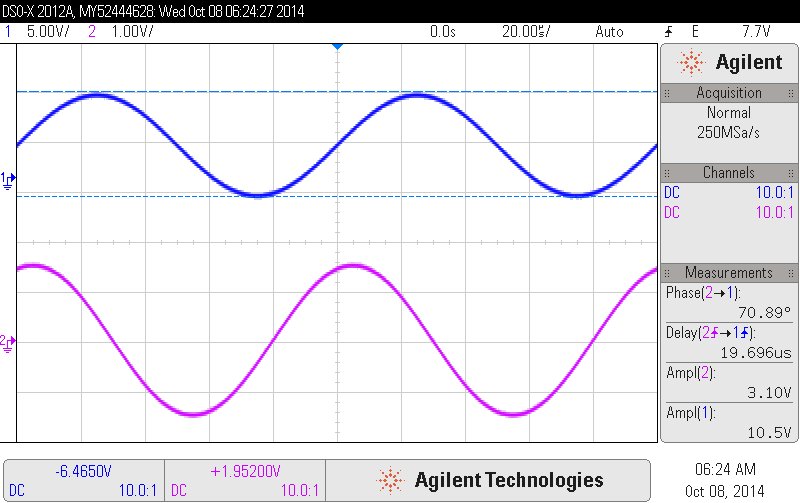
\includegraphics[width=0.475\textwidth]{scope_0}} \quad
		\subfigure[5 k$\Omega$]{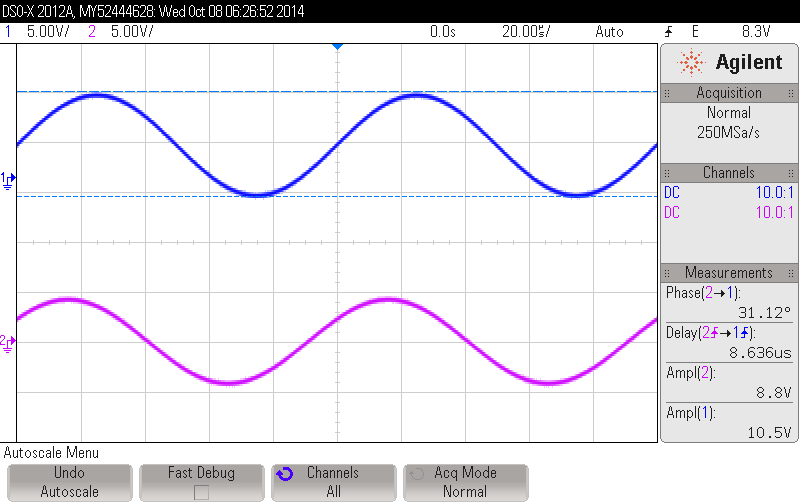
\includegraphics[width=0.475\textwidth]{scope_1}}
		\subfigure[10 k$\Omega$]{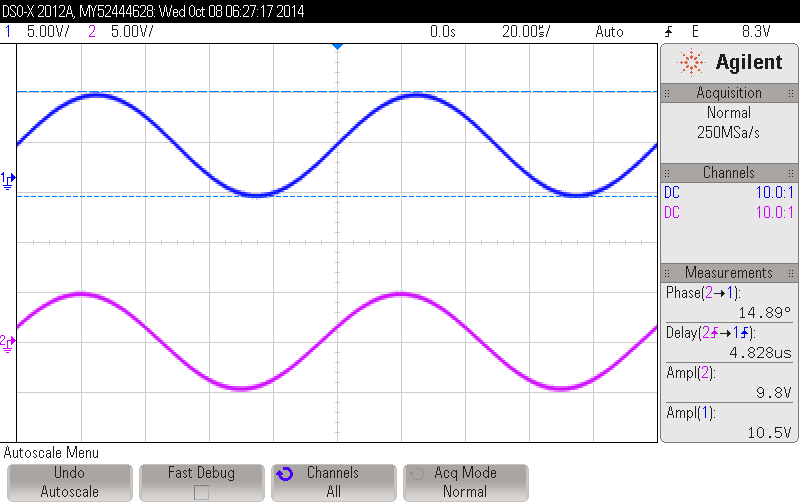
\includegraphics[width=0.475\textwidth]{scope_2}}
	\caption{RC circuit measurements}
	\label{fig:rc_meas}
\end{sidewaysfigure}

\pagebreak

\begin{sidewaysfigure}
	\centering	
		\subfigure[1 $\mu$H]{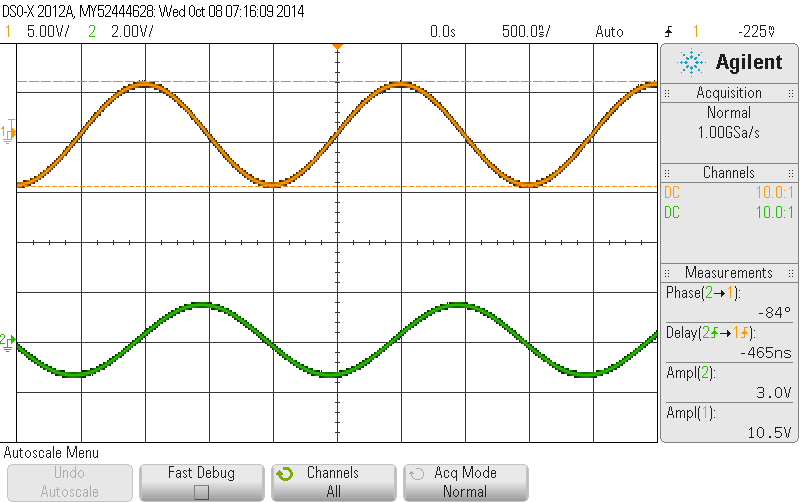
\includegraphics[width=0.475\textwidth]{scope_3}} \quad
		\subfigure[220 $\mu$H]{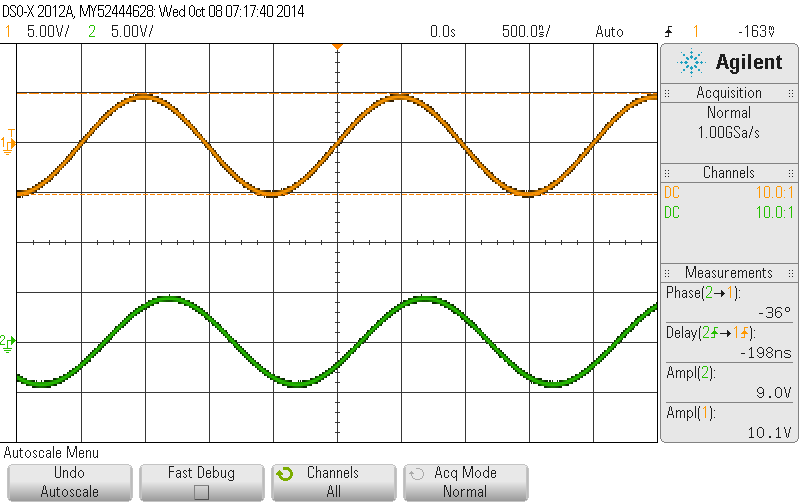
\includegraphics[width=0.475\textwidth]{scope_6}} \quad
		\subfigure[470 $\mu$H]{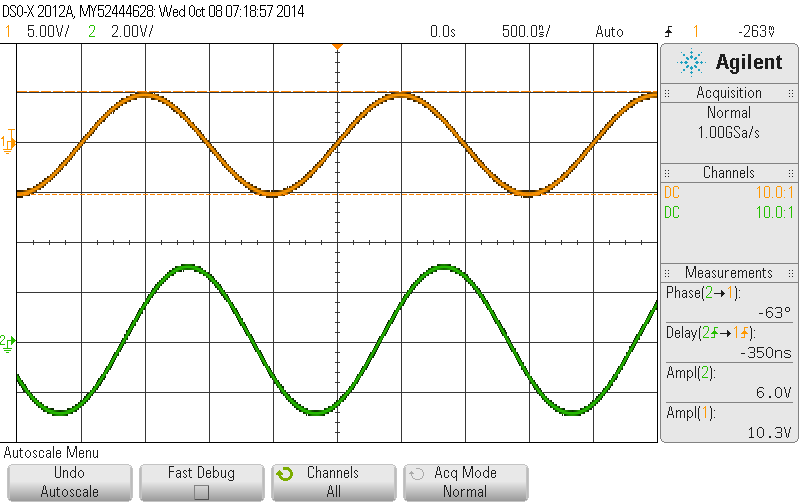
\includegraphics[width=0.475\textwidth]{scope_9}} \quad
		\subfigure[1000 $\mu$H]{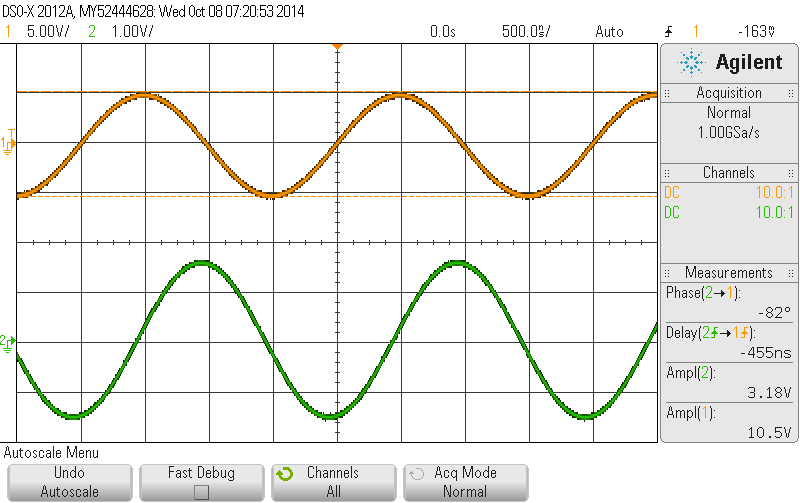
\includegraphics[width=0.475\textwidth]{scope_12}}
	\caption{RL circuit measurements for 1 k$\Omega$ resistor}
	\label{fig:rl_meas_1k}
\end{sidewaysfigure}

\pagebreak

\begin{sidewaysfigure}
	\centering	
		\subfigure[1 $\mu$H]{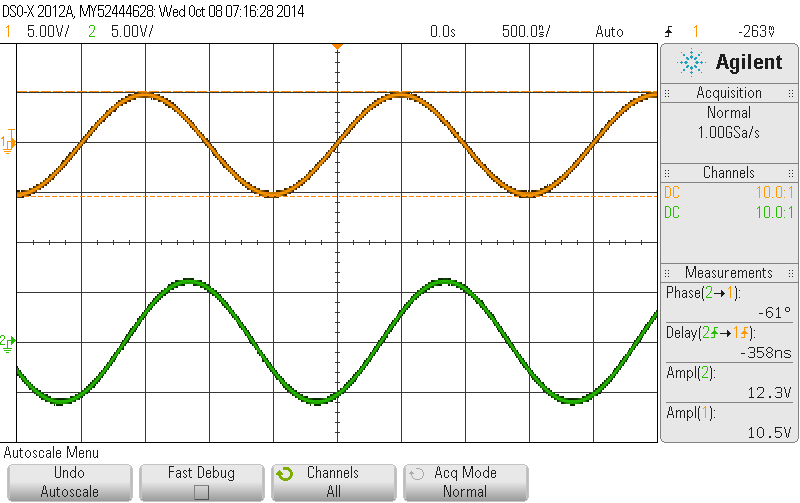
\includegraphics[width=0.475\textwidth]{scope_4}} \quad
		\subfigure[220 $\mu$H]{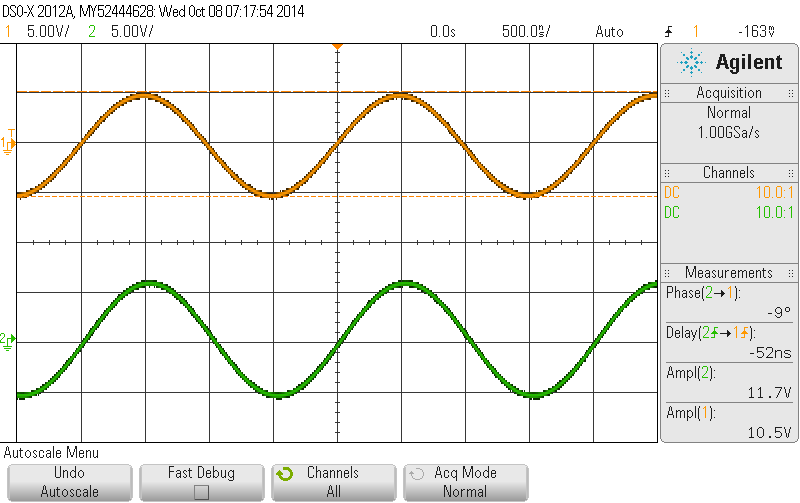
\includegraphics[width=0.475\textwidth]{scope_7}} \quad
		\subfigure[470 $\mu$H]{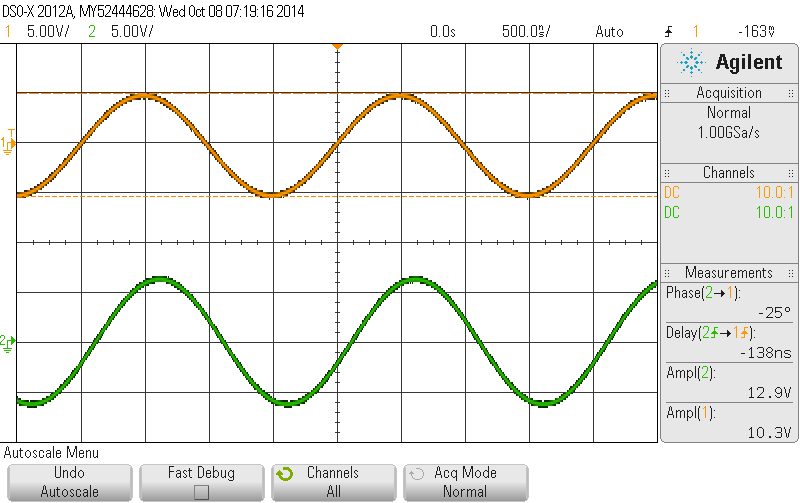
\includegraphics[width=0.475\textwidth]{scope_10}} \quad
		\subfigure[1000 $\mu$H]{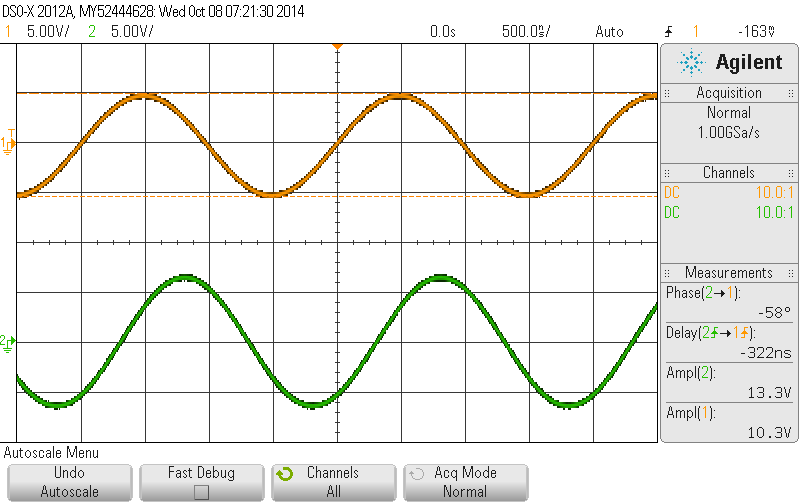
\includegraphics[width=0.475\textwidth]{scope_13}}
	\caption{RL circuit measurements for 5 k$\Omega$ resistor}
	\label{fig:rl_meas_5k}
\end{sidewaysfigure}

\pagebreak

\begin{sidewaysfigure}
	\centering	
		\subfigure[1 $\mu$H]{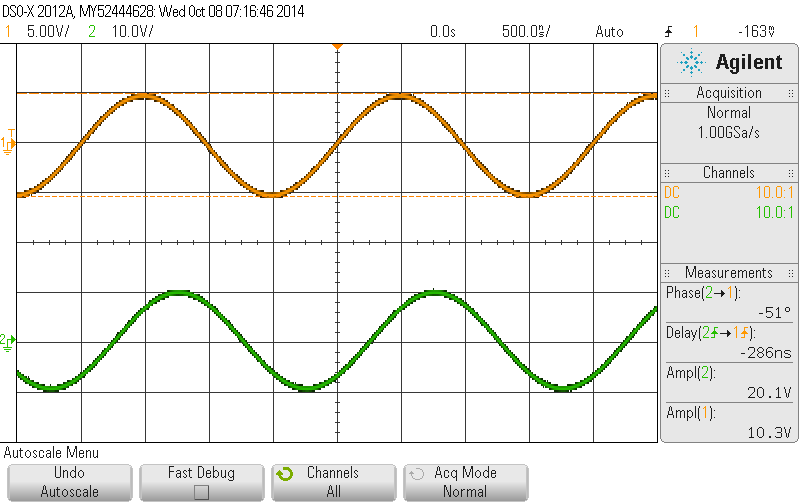
\includegraphics[width=0.475\textwidth]{scope_5}} \quad
		\subfigure[220 $\mu$H]{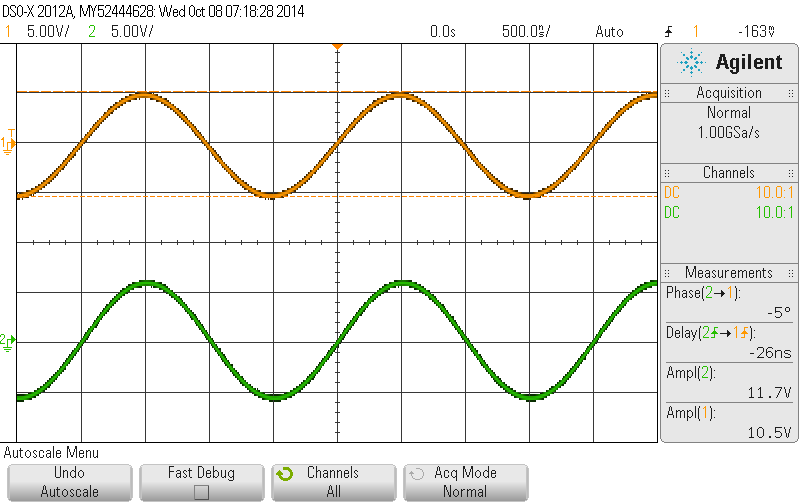
\includegraphics[width=0.475\textwidth]{scope_8}} \quad
		\subfigure[470 $\mu$H]{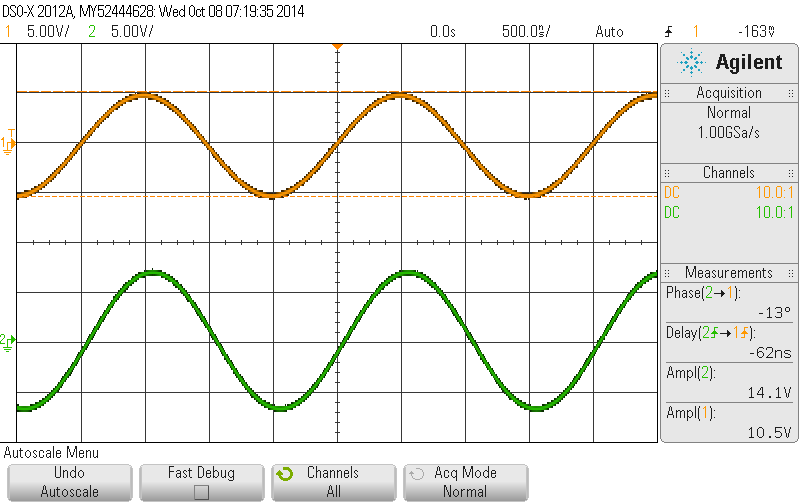
\includegraphics[width=0.475\textwidth]{scope_11}} \quad
		\subfigure[1000 $\mu$H]{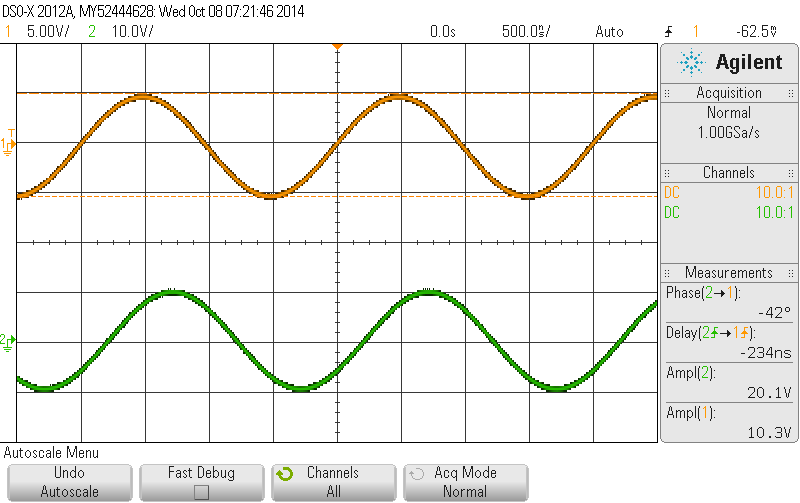
\includegraphics[width=0.475\textwidth]{scope_14}}
	\caption{RL circuit measurements for 10 k$\Omega$ resistor}
	\label{fig:rl_meas_10k}
\end{sidewaysfigure}

%----------------------------------------------------------------------------
%----------------------------------------------------------------------------
%			DO NOT DELETE BELOW
%----------------------------------------------------------------------------
%----------------------------------------------------------------------------

\end{document}